% DPF 09 talk on strangeness in nucleon

\documentclass[10pt]{beamer}
\usepackage{amsmath}
\usepackage{mathtools}
%\documentclass[12pt]{beamerthemeSam.sty}
\usepackage{epsf}
%\usepackage{pstricks}
%\usepackage[orientation=portrait,size=A4]{beamerposter}
\geometry{paperwidth=160mm,paperheight=120mm}
%DT favorite definitions
\def\LL{\left\langle}	% left angle bracket
\def\RR{\right\rangle}	% right angle bracket
\def\LP{\left(}		% left parenthesis
\def\RP{\right)}	% right parenthesis
\def\LB{\left\{}	% left curly bracket
\def\RB{\right\}}	% right curly bracket
\def\PAR#1#2{ {{\partial #1}\over{\partial #2}} }
\def\PARTWO#1#2{ {{\partial^2 #1}\over{\partial #2}^2} }
\def\PARTWOMIX#1#2#3{ {{\partial^2 #1}\over{\partial #2 \partial #3}} }

\def\rightpartial{{\overrightarrow\partial}}
\def\leftpartial{{\overleftarrow\partial}}
\def\diffpartial{\buildrel\leftrightarrow\over\partial}

\def\BI{\begin{itemize}}
\def\EI{\end{itemize}}
\def\BE{\begin{displaymath}}
\def\EE{\end{displaymath}}
\def\BEA{\begin{eqnarray*}}
\def\EEA{\end{eqnarray*}}
\def\BNEA{\begin{eqnarray}}
\def\ENEA{\end{eqnarray}}
\def\EL{\nonumber\\}


\newcommand{\map}[1]{\frame{\frametitle{\textbf{Course map}}
\centerline{\includegraphics[height=0.86\paperheight]{../../map/#1.png}}}}
\newcommand{\wmap}[1]{\frame{\frametitle{\textbf{Course map}}
\centerline{\includegraphics[width=0.96\paperwidth]{../../map/#1.png}}}}

\newcommand{\etal}{{\it et al.}}
\newcommand{\gbeta}{6/g^2}
\newcommand{\la}[1]{\label{#1}}
\newcommand{\ie}{{\em i.e.\ }}
\newcommand{\eg}{{\em e.\,g.\ }}
\newcommand{\cf}{cf.\ }
\newcommand{\etc}{etc.\ }
\newcommand{\atantwo}{{\rm atan2}}
\newcommand{\Tr}{{\rm Tr}}
\newcommand{\dt}{\Delta t}
\newcommand{\op}{{\cal O}}
\newcommand{\msbar}{{\overline{\rm MS}}}
\def\chpt{\raise0.4ex\hbox{$\chi$}PT}
\def\schpt{S\raise0.4ex\hbox{$\chi$}PT}
\def\MeV{{\rm Me\!V}}
\def\GeV{{\rm Ge\!V}}

%AB: my color definitions
%\definecolor{mygarnet}{rgb}{0.445,0.184,0.215}
%\definecolor{mygold}{rgb}{0.848,0.848,0.098}
%\definecolor{myg2g}{rgb}{0.647,0.316,0.157}
\definecolor{abtitlecolor}{rgb}{0.0,0.255,0.494}
\definecolor{absecondarycolor}{rgb}{0.0,0.416,0.804}
\definecolor{abprimarycolor}{rgb}{1.0,0.686,0.0}
\definecolor{Red}           {cmyk}{0,1,1,0}
\definecolor{Grey}           {cmyk}{.7,.7,.7,0}
\definecolor{Lg}           {cmyk}{.4,.4,.4,0}
\definecolor{Blue}          {cmyk}{1,1,0,0}
\definecolor{Green}         {cmyk}{1,0,1,0}
\definecolor{Brown}         {cmyk}{0,0.81,1,0.60}
\definecolor{Black}         {cmyk}{0,0,0,1}

\usetheme{Madrid}


%AB: redefinition of beamer colors
%\setbeamercolor{palette tertiary}{fg=white,bg=mygarnet}
%\setbeamercolor{palette secondary}{fg=white,bg=myg2g}
%\setbeamercolor{palette primary}{fg=black,bg=mygold}
\setbeamercolor{title}{fg=abtitlecolor}
\setbeamercolor{frametitle}{fg=abtitlecolor}
\setbeamercolor{palette tertiary}{fg=white,bg=abtitlecolor}
\setbeamercolor{palette secondary}{fg=white,bg=absecondarycolor}
\setbeamercolor{palette primary}{fg=black,bg=abprimarycolor}
\setbeamercolor{structure}{fg=abtitlecolor}

\setbeamerfont{section in toc}{series=\bfseries}

%AB: remove navigation icons
\beamertemplatenavigationsymbolsempty
\title{
  \textbf {Rotational motion}\\
%\centerline{}
%\centering
%\vspace{-0.0in}
%\includegraphics[width=0.3\textwidth]{propvalues_0093.pdf}
%\vspace{-0.3in}\\
%\label{intrograph}
}

\author[W. Freeman] {Physics 211\\Syracuse University, Physics 211 Spring 2015\\Walter Freeman}

\date{\today}

\begin{document}

\frame{\titlepage}

\frame{\frametitle{\textbf{Announcements}}
\BI
\item{Homework due Wednesday; next homework due next Wednesday}
\item{Next Mastering Physics assignment will be posted tonight and will be due next Tuesday before class}
\EI
}

\frame{\frametitle{\textbf{Ask a Physicist: Dark matter}}
}

\frame{\frametitle{\textbf{Rotational motion}}
  \BI
\item{This week we're going to redo everything that we've done so far}
\item{Everything you've learned about linear motion has a rotational equivalent}
  \BI
\item{Position, velocity, acceleration $\leftrightarrow$ angle, angular velocity, angular acceleration}
\item{Kinematics for coordinates  $\leftrightarrow$ kinematics for angles}
\item{Newton's second law $\leftrightarrow$ Newton's law for rotation}
\item{Force  $\leftrightarrow$ torque}
\item{Mass  $\leftrightarrow$ moment of inertia}
\item{... and others}
  \EI
  \EI
}

\frame{\frametitle{\textbf{The plan for this week}}
  \large
  \BI
\item{I'm going to go over all of the concepts for rotational motion, rather quickly}
\item{These concepts are mostly directly analogous to those you already know}
\item{This will serve as a reference for you: find the slides online, or take notes}
\item{Then we'll stop, slow down, do lots of demos and examples}
 \item{This material is historically difficult for students, but it doesn't need to be}
   \pause
 \item{\color{Red}Here we go: we're going to recap the entire course!}
 \EI
}

\frame{\frametitle{\textbf{Our task}}
\BI
\item{We have so far studied the motion of ``pointlike'' objects}
  \BI
\item{``This object is located at this position''}
  \EI
\item{Now we're going to consider extended objects}
\item{They can move around, using the physics ($\vec F = m \vec a$, etc.) that you already know}
  \pause
\item{... but they can also {\it rotate}}
  \centerline{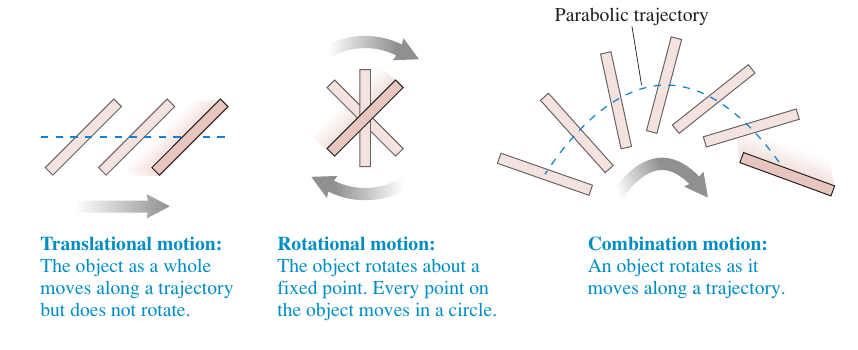
\includegraphics[width=0.5\textwidth]{rotation.png}}
\item{Rotation is the new thing, so let's study it!}
  \pause
\item{\color{Red}It turns out rotation in many of the same ways as translation: this is really review!}
  \EI
}
 
\frame{\frametitle{\textbf{Describing rotation}}
  \BI
\item{In the first section we were concerned about $x(t)$ and $y(t)$ -- the components of the displacement vector}
\item{\color{Red}Here we're concerned about angle as a function of time: $\theta(t)$}
  \BI
\item{In two dimensions angle is a scalar: no funny vectors!}
\item{By convention: clockwise is negative, counterclockwise is positive}
  \EI
\item{We gave names to the derivatives of position: ``velocity'' and ``acceleration''}
\item{Likewise, we give names to the derivatives of angle}
  \BI
\item{$\omega \equiv \PAR{\theta}{t}$: ``angular velocity'', measured in rad/s (you knew this!)}
\item{$\alpha \equiv \PARTWO{\theta}{t}$: ``angular acceleration'', measured in rad/$s^2$ (new!)}
  \EI
  \EI
}

\frame{\frametitle{\textbf{Going from rotation to translation}}
  \BI
\item{``If an object is turning at some angular velocity $\omega$, how fast is a piece at radius $r$ moving?''}
\item{We did this before: remember the tangential velocity $v_T = \omega r$, based on the definition of the radian}
\item{This holds true for all of the derivatives of angle and position:}
  \Large
\item{Arc length: \color{Red}$s = \theta r$}
\item{Tangential velocity: \color{Red} $v_T = \omega r$}
\item{Tangential acceleration: \color{Red} $a_T = \alpha r$}

  \pause
  \bigskip
  \bigskip

\item{To go from rotational descriptions of motion to tangential ones, multiply by the radius}
\EI
}

\frame{\frametitle{\textbf{Rotational kinematics}}
\BI
\item{The constant-acceleration kinematics we learned was really about {\it the relation of a function to its derivatives}}
\item{Since the same derivative relationships hold, the exact same kinematics applies:}
\EI

\bigskip

    \large
\centerline{  \begin{tabular}{| c | c |}
    \hline
    Translation & Rotation \\
    \hline
    \hline
    \hline
    Position $x$ & Angle $\theta$ \\
    \hline
    Velocity $v$ & Angular velocity $\omega$ \\
    \hline
    Acceleration $a$ & Angular acceleration $\alpha$ \\
    \hline
    \hline
    $v(t) = v_0 + at$ & $\omega(t) = \omega_0 + \alpha t$ \\
    \hline
    $x(t) = x_0 + v_0 t + \frac{1}{2}at^2$ & $\theta(t) = \theta_0 + \omega_0 t + \frac{1}{2} \alpha t^2$ \\
    \hline
    $v_f^2 - v_0^2 = 2a \Delta x$ & $ \omega_f^2 - \omega_0^2 = 2 \alpha \Delta \theta$ \\
    \hline
  \end{tabular}
}

\bigskip

\centerline{Relate $\theta$, $\omega$, $\alpha$, and $t$ the same way you do $x$, $v$, $a$, and $t$}

\bigskip

\centerline{Note that one revolution = 360 degrees = $2\pi$ radians!}
}


\frame{\frametitle{\textbf{What corresponds to Newton's second law?}}
  \Large
  \centerline{The key idea in translational motion is Newton's second law $\vec F = m \vec a$.}


  \bigskip
  \bigskip

  \pause

  \centerline{What is the corresponding idea for rotational motion?}

\bigskip
\bigskip

  \BI
\item{Angular acceleration $\alpha$ corresponds to $\vec a$}
\item{The rotational analogue of force is called {\bf \color{Red} torque}}
\item{The rotational analogue of mass is called {\bf \color{Red} moment of inertia}}
  \EI
  \bigskip
  \bigskip

  \pause

  \centerline{Let's look at each of those in turn.}

}

\frame{\frametitle{\textbf{Torque}}
  \Large
  \centerline{Torque ($\tau$) is the rotational analogue of force: ``rotational push or pull''}

  \BI
  \large
\item{Forces applied to an object result in torques: ``push on something to turn it''}
\item{The size of the torque depends on three things:}
  \pause
\item{The size of the force}
  \BI
\item{Push harder to exert more torque -- that's easy!}
  \EI
  \pause
\item{The distance from the force to the pivot point}
  \BI
\item{The further from the pivot to the point of force, the greater the torque}
\item{This is why the door handle is on the outside of the door...}
  \EI
\item{The angle at which the force is applied}
  \BI
\item{Only forces ``in the direction of rotation'' make something turn}
\item{The torque depends only on the {\it component of the force perpendicular to the radius}}
  \EI
  \EI
}
\frame{\frametitle{\textbf{Computing torque}}
  \centerline{\Huge $\tau = F_\perp r$}
\begin{center}
\Large Torque is equal to the distance from the pivot, \\times the perpendicular component of the force
\end{center}


  \centerline{\color{Lg}(There is an equivalent alternative we will see a bit later)}
\bigskip
  \centerline{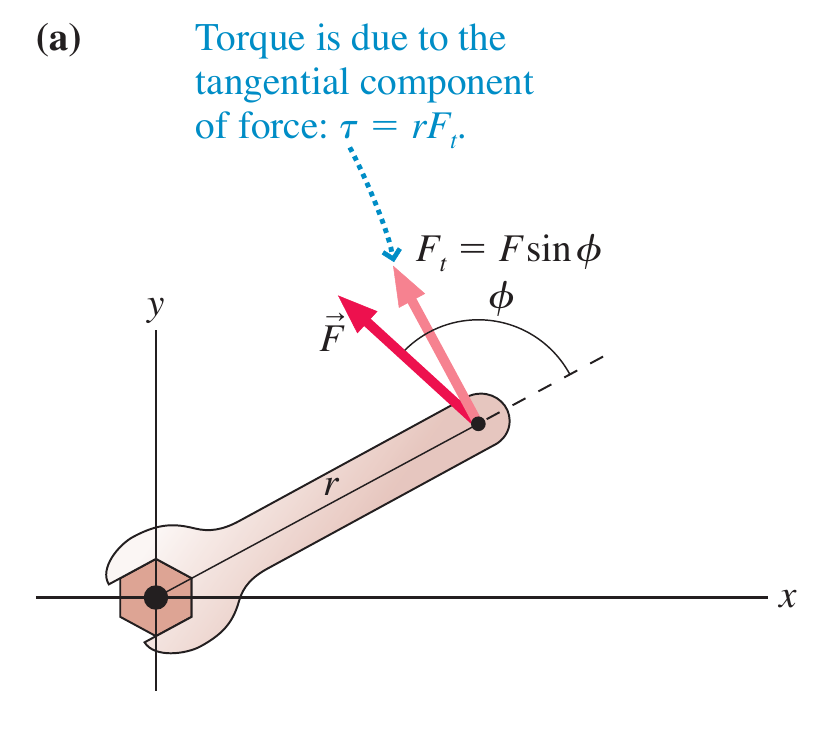
\includegraphics[width=0.3\textwidth]{torque1.png}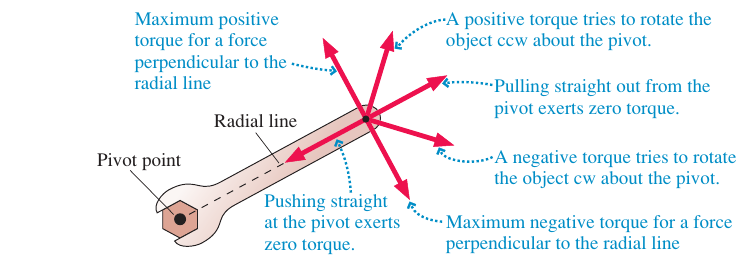
\includegraphics[width=0.6\textwidth]{torque2.png}}

\bigskip

  \centerline{Note that torque has a sign, just like angular velocity: CCW is positive; CW is negative.}
}

\frame{\frametitle{\textbf{Important notes about torque}}
  \centerline{\Large These are very important: note them somewhere for later reference!}
  \bigskip
  \bigskip
  \BI
\item{Torques are in reference to a {\bf particular pivot}}
\item{This is different from force; if you're talking about torque, you {\it must} say what axis it's measured around}
\item{Torque now depends on the {\it location} of forces, not just their size}
\BI
\item{Your force diagrams now need to show the place where forces act!}
\item{Weight acts at the center of mass (``the middle''); we'll see what that means later}
\item{A saimple force diagram might look like this:}
  
  \bigskip
  
  \centerline{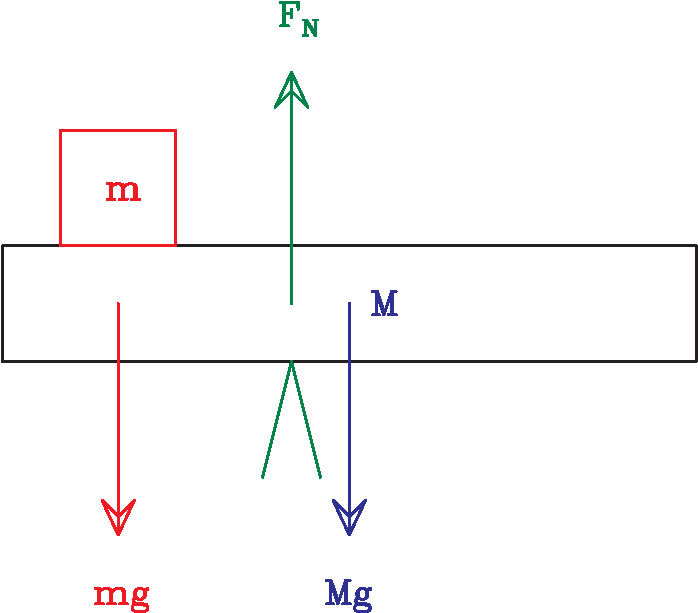
\includegraphics[width=0.3\textwidth]{diag-crop.pdf}}
  \EI
\EI
  }

\frame{\frametitle{\textbf{What about the mass analogue?}}
  \centerline{\Huge $\vec F = m \vec a$}

\medskip

  \centerline{\Huge $\tau =\, ? \alpha$}

  \bigskip
  \bigskip
  \bigskip

  \centerline{\Large Mass tells you how hard it is to give something a (linear) acceleration.}
  \centerline{\Large What determines how hard something is to turn?}
  
  \bigskip
  \bigskip
  \bigskip

\centerline{\Large We can already look at situations where $\tau=\alpha=0$: ``static equilibrium''}
}

\frame{\frametitle{\textbf{Moment of inertia}}
  \centerline{\Large The analogue of mass is called ``moment of inertia'' (letter $I$)}
  
  \BI
  \large
\item{More massive things are harder to turn, but that's only part of it}
\item{The mass {\it distribution} matters, too}
\item{The further the mass is from the center, the harder it will be to turn}
\item{The moment of inertia depends on the {\it average squared distance from the center}}
    \BI
  \item{\color{Lg}I state this without proof here; if you're interested in why, come see me!}
    \EI
  \EI

  \bigskip\pause

  \centerline{\Large $I=MR^2$}

\bigskip
\bigskip
\bigskip

  \centerline{\large (if all the mass is the same distance from the center)}
  \centerline{\large (our demo rods; hoops; rings; bike wheels)} 
}

\frame{\frametitle{\textbf{Moment of inertia, other things}}
  \centerline{\Large What about the moment of inertia of other objects?}
  \centerline{\large Requires calculus in general; here are some common ones} 
  \centerline{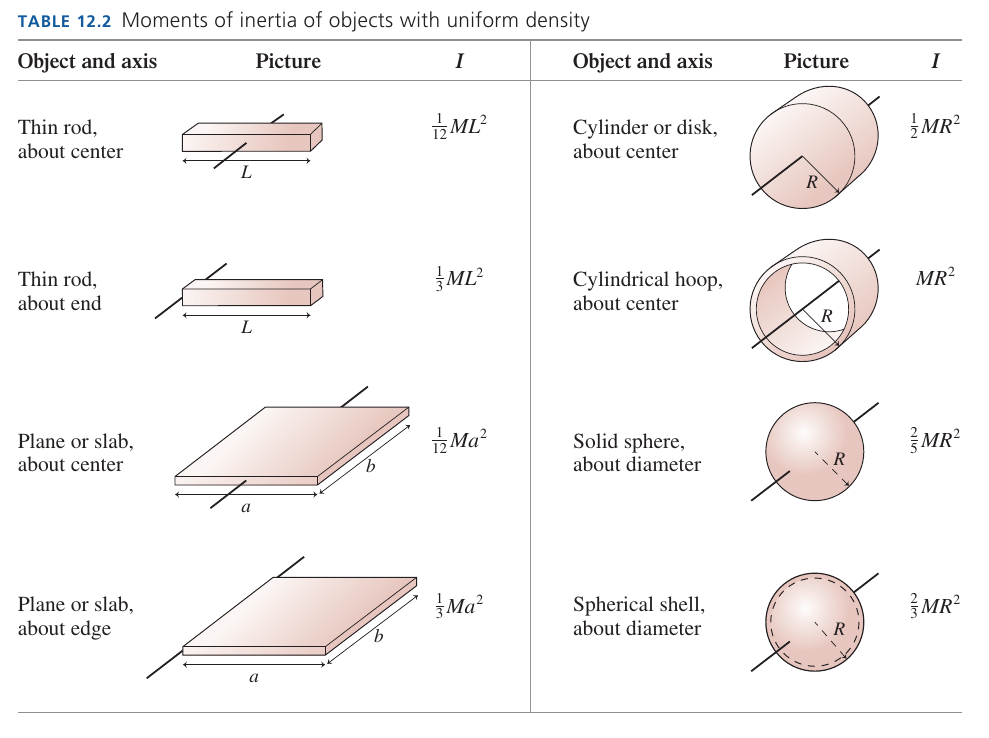
\includegraphics[width=0.7\textwidth]{moment-table.png}}
  }

  \frame{\frametitle{\textbf{Putting it together: Newton's law for rotation}}
    \centerline{
  \begin{tabular}{| c | c |}
    \hline
    Translation & Rotation \\
    \hline
    \hline
    \hline
    Force $\vec F$ & Torque: $\tau=F_\perp r$ \\
    \hline
    Mass $m$ & Moment of Inertia: $I = \lambda MR^2$ \\
    \hline
    Acceleration $\vec a$ & Angular acceleration $\alpha$ \\
    \hline
    \hline
    $\vec F = m \vec a$ & $\tau = I \alpha$ \\
    \hline
  \end{tabular}
}

\bigskip
\bigskip
\bigskip

\centerline{\Large This last line can be thought of as ``Newton's second law for rotation''.}
\bigskip
\bigskip
\bigskip
\centerline{\large Torques give things angular acceleration, just like forces make things accelerate:}
\bigskip
\centerline{\Huge $\tau = I \alpha$}
}

\frame{\frametitle{\textbf{What about energy?}}

  We saw before that the work-energy theorem was just a consequence of the ``third kinematics relation''.
  Is there anything that corresponds to this for rotation?

  \bigskip
  \bigskip
  \bigskip
  \pause

  \centerline{\Large \color{Red} Yes, and it's exactly what you'd expect!}
  \centerline{
  \begin{tabular}{| c | c |}
    \hline
    Translation & Rotation \\
    \hline
    \hline
    \hline
    Force $\vec F$ & Torque: $\tau=F_\perp r$ \\
    \hline
    Mass $m$ & Moment of Inertia: $I = \lambda MR^2$ \\
    \hline
    Displacement $\vec s$ & Angular displacement $\theta$ \\
    \hline
    Velocity $\vec v$ & Angular velocity $\omega$ \\
    \hline
    \hline
    Work = $\vec F \cdot \Delta \vec s$ & Work = $\tau \Delta \theta$ \\
    \hline
    Kinetic energy $\frac{1}{2} mv^2$ & Kinetic energy $\frac{1}{2} I \omega^2$ \\
    \hline
  \end{tabular}
}

\bigskip
\bigskip
\bigskip

\centerline{\Large There is rotational kinetic energy $\frac{1}{2} I \omega^2$ associated with spinning objects!}
\centerline{\large This is just another term to add to your conservation of energy relations!}

}

\frame{\frametitle{\textbf{What about momentum?}}
\centerline{
  \begin{tabular}{| c | c |}
    \hline
    Translation & Rotation \\
    \hline
    \hline
    \hline
    Mass $m$ & Moment of Inertia: $I = \lambda MR^2$ \\
    \hline
    Velocity $\vec v$ & Angular velocity $\omega$ \\
    \hline
    \hline
    Momentum $\vec p = m \vec v$ & Angular momentum $L = I \omega$ \\
    \hline
  \end{tabular}
}

\bigskip
\bigskip
\bigskip

Just as momentum is conserved in the absence of external forces, angular momentum is conserved in the absence of external torques.

}
\end{document}
